%%%%%%%%%%%%%%%%%%%%%%%%%%%%% Define Article %%%%%%%%%%%%%%%%%%%%%%%%%%%%%%%%%%
\documentclass{article}
\setcounter{secnumdepth}{3} % Establecer nivel de profundidad para las subsubsecciones en el índice
%%%%%%%%%%%%%%%%%%%%%%%%%%%%%%%%%%%%%%%%%%%%%%%%%%%%%%%%%%%%%%%%%%%%%%%%%%%%%%%

%%%%%%%%%%%%%%%%%%%%%%%%%%%%% Using Packages %%%%%%%%%%%%%%%%%%%%%%%%%%%%%%%%%%
\usepackage{geometry}
\usepackage{graphicx}
\usepackage{amssymb}
\usepackage{amsmath}
\usepackage{amsthm}
\usepackage{empheq}
\usepackage{mdframed}
\usepackage{booktabs, tabularx, wrapfig}
\usepackage{lipsum}
\usepackage{color}
\usepackage{psfrag}
\usepackage{pgfplots}
\usepackage{bm}
\usepackage[spanish]{babel}
\usepackage{biblatex}
\usepackage{csquotes}
\usepackage[hidelinks]{hyperref}
\usepackage{caption}
\usepackage{tocloft}
\usepackage{float}
\usepackage{dirtytalk}
%%%%%%%%%%%%%%%%%%%%%%%%%%%%%%%%%%%%%%%%%%%%%%%%%%%%%%%%%%%%%%%%%%%%%%%%%%%%%%%

% Other Settings

%%%%%%%%%%%%%%%%%%%%%%%%%% Page Setting %%%%%%%%%%%%%%%%%%%%%%%%%%%%%%%%%%%%%%%
\geometry{
    left=2cm,
    right=2cm,
    top=2cm,
    bottom=2cm
}
\graphicspath{{/img/}}
\addbibresource{bibliography.bib}
\hypersetup{hidelinks}
\addto\captionsspanish{
  \renewcommand{\listtablename}{Índice de Tablas}
}

%%%%%%%%%%%%%%%%%%%%%%%%%% Define some useful colors %%%%%%%%%%%%%%%%%%%%%%%%%%
\definecolor{ocre}{RGB}{243,102,25}
\definecolor{mygray}{RGB}{243,243,244}
\definecolor{deepGreen}{RGB}{26,111,0}
\definecolor{shallowGreen}{RGB}{235,255,255}
\definecolor{deepBlue}{RGB}{61,124,222}
\definecolor{shallowBlue}{RGB}{235,249,255}
%%%%%%%%%%%%%%%%%%%%%%%%%%%%%%%%%%%%%%%%%%%%%%%%%%%%%%%%%%%%%%%%%%%%%%%%%%%%%%%

%%%%%%%%%%%%%%%%%%%%%%%%%% Define an orangebox command %%%%%%%%%%%%%%%%%%%%%%%%
\newcommand\orangebox[1]{\fcolorbox{ocre}{mygray}{\hspace{1em}#1\hspace{1em}}}
%%%%%%%%%%%%%%%%%%%%%%%%%%%%%%%%%%%%%%%%%%%%%%%%%%%%%%%%%%%%%%%%%%%%%%%%%%%%%%%

%%%%%%%%%%%%%%%%%%%%%%%%%%%% English Environments %%%%%%%%%%%%%%%%%%%%%%%%%%%%%
\newtheoremstyle{mytheoremstyle}{3pt}{3pt}{\normalfont}{0cm}{\rmfamily\bfseries}{}{1em}{{\color{black}\thmname{#1}~\thmnumber{#2}}\thmnote{\,--\,#3}}
\newtheoremstyle{myproblemstyle}{3pt}{3pt}{\normalfont}{0cm}{\rmfamily\bfseries}{}{1em}{{\color{black}\thmname{#1}~\thmnumber{#2}}\thmnote{\,--\,#3}}
\theoremstyle{mytheoremstyle}
\newmdtheoremenv[linewidth=1pt,backgroundcolor=shallowGreen,linecolor=deepGreen,leftmargin=0pt,innerleftmargin=20pt,innerrightmargin=20pt,]{theorem}{Theorem}[section]
\theoremstyle{mytheoremstyle}
\newmdtheoremenv[linewidth=1pt,backgroundcolor=shallowBlue,linecolor=deepBlue,leftmargin=0pt,innerleftmargin=20pt,innerrightmargin=20pt,]{definition}{Definition}[section]
\theoremstyle{myproblemstyle}
\newmdtheoremenv[linecolor=black,leftmargin=0pt,innerleftmargin=10pt,innerrightmargin=10pt,]{problem}{Problem}[section]
%%%%%%%%%%%%%%%%%%%%%%%%%%%%%%%%%%%%%%%%%%%%%%%%%%%%%%%%%%%%%%%%%%%%%%%%%%%%%%%

%%%%%%%%%%%%%%%%%%%%%%%%%%%%%%% Plotting Settings %%%%%%%%%%%%%%%%%%%%%%%%%%%%%
\usepgfplotslibrary{colorbrewer}
\pgfplotsset{width=8cm,compat=1.9}
%%%%%%%%%%%%%%%%%%%%%%%%%%%%%%%%%%%%%%%%%%%%%%%%%%%%%%%%%%%%%%%%%%%%%%%%%%%%%%%


\begin{document}
%%%%%%%%%%%%%%%%%%%%%%%%%%%%%%% Title & Author %%%%%%%%%%%%%%%%%%%%%%%%%%%%%%%%
    \begin{titlepage}
    \begin{figure}[h]
        \centering
        
\includegraphics[width=2.06111in,height=1.68611in]{img/image1.png}
    \end{figure}

    \begin{center}
        \LARGE
        FACULTAD DE INGENIERÍA
        MAGISTER EN GESTIÓN DE TECNOLOGÍAS DE LA INFORMACIÓN Y TELECOMUNICACIONES

        
        \Huge
        \textbf{Análisis de la relación entre la resolución de una guía de programación y el éxito académico en el ramo de introducción a la programación}


        \LARGE
        Un enfoque predictivo utilizando redes bayesianas        


        \textbf{Autor}\\
        Gaston Ernesto Sepulveda Espinoza


        \textbf{Profesor Guía}\\
        Billy Mark Peralta Márquez

        \begin{flushright}
            TRABAJO DE TESIS PRESENTADO EN CONFORMIDAD 
            A LOS REQUISITOS PARA OBTENER EL GRADO DE 
            MAGISTER EN GESTIÓN DE TECNOLOGÍAS DE LA INFORMACIÓN Y TELECOMUNICACIONES
        \end{flushright}


        \Large
        Santiago, Chile 2023         

    \end{center}
\end{titlepage}
%%%%%%%%%%%%%%%%%%%%%%%%%%%%%%%%%%%%%%%%%%%%%%%%%%%%%%%%%%%%%%%%%%%%%%%%%%%%%%%

%%%%%%%%%%%%%%%%%%%%%%%%%%%%%%% Body %%%%%%%%%%%%%%%%%%%%%%%%%%%%%%%%
    % \tableofcontents

\begin{center}
    \textbf{\LARGE AGRADECIMIENTO}
\end{center}

En primera instancia agradezco a …
\vfill


\begin{center}
    \textbf{\LARGE \textit{Título}}
\end{center}

Nombre Completo Alumno/a

Bajo la supervisión del Profesor <Nombre Profesor/a> en la Universidad Andrés Bello

\begin{center}
    \textbf{\LARGE \textit{Resumen}}
\end{center}
En este trabajo se examina si la resolución de una guía de programación 
está relacionada con el éxito académico en el ramo de introducción a la 
programación en la Universidad Andrés Bello. Se investiga si la guía, que 
consta de 52 ejercicios y no es obligatoria, ayuda a los estudiantes 
a enfrentar la primera prueba del ramo y si puede predecir la deserción 
en la carrera. 
Además, se propone el uso de redes bayesianas para generar predicciones 
sobre su relevancia para aprobar el ramo y su capacidad predictiva para 
la deserción. El estudio incluye una revisión bibliográfica sobre estudios 
previos relacionados, un análisis descriptivo de los datos recolectados y 
una discusión sobre las implicaciones prácticas y teóricas del estudio. 
Los resultados sugieren que resolver la guía puede estar relacionado con 
el éxito académico y pueden ser útiles para predecir la deserción en el ramo.

\tableofcontents

\hypertarget{Introducción}{%
    \section{Introducción}\label{Introducción}}
    \vfill
La programación es una habilidad cada vez más demandada en el mercado laboral
 y es fundamental para el desarrollo de la tecnología. 
Por esta razón, muchas universidades ofrecen cursos de introducción a la 
programación para formar a los futuros profesionales en esta área. 
Sin embargo, algunos estudiantes pueden tener dificultades para aprobar estos 
cursos debido a la complejidad de los conceptos y la falta de experiencia 
previa en programación. 
Para ayudar a los estudiantes a enfrentar estos desafíos, algunas 
universidades ofrecen guías de programación que contienen ejercicios y 
problemas para resolver. 
En este contexto, surge la pregunta: 
¿la resolución de una guía de programación está relacionada con el éxito 
académico en el ramo de introducción a la programación? 
Este trabajo examina esta cuestión en el contexto de la 
Universidad Andrés Bello y propone el uso de redes bayesianas para generar 
predicciones sobre su relevancia para aprobar el ramo y su capacidad 
predictiva para la deserción. 
Los resultados pueden ser útiles para mejorar las estrategias de apoyo a 
los estudiantes y la toma de decisiones en relación con las guías como 
recurso educativo.
\vfill

\hypertarget{Fundamentación}{%
\section{Fundamentación}\label{Fundamentación}}

La educación superior en informática y programación trasciende las demandas del mercado laboral, reflejando cómo la tecnología está transformando nuestra sociedad. En este escenario, la programación no solo se presenta como una habilidad técnica, sino también como un enfoque de pensamiento y resolución de problemas.

La educación superior, particularmente en campos técnicos como la informática, es crucial para cultivar profesionales capaces de navegar y adaptarse a las vertiginosas transformaciones tecnológicas. Hair, Black, Babin, Anderson, \& Tatham (2019) \cite{hair2019advanced} enfatizan que la educación superior es fundamental para formar individuos equipados para los retos del mundo actual. No obstante, debido a su naturaleza abstracta y lógica, la programación puede representar un desafío considerable para muchos estudiantes.

Las guías de programación sirven como nexos entre la teoría y la aplicación. Han, Kamber, \& Pei (2011) \cite{han2011data} y García, Romero, \& Ventura (2018) \cite{garcia2018prediccion} sostienen que, al proporcionar ejercicios prácticos y contextualizados, estas guías son vitales para consolidar el aprendizaje teórico y práctico, preparando a los estudiantes para evaluaciones y situaciones reales.

En una era dominada por la data, las técnicas convencionales de análisis ya no bastan. Las redes bayesianas, descritas por Koller y Friedman (2009) \cite{koller2009introduction}, ofrecen una visión más enriquecida, permitiendo modelar la incertidumbre y las interacciones entre variables, lo que es crucial para entender las dinámicas inherentes al aprendizaje.

La interpretabilidad de los modelos ha cobrado importancia en tiempos recientes. La demanda de modelos claros y comprensibles es primordial, sobre todo en el contexto educativo. Lipton (2018) \cite{lipton2018mythos} y Doshi-Velez \& Kim (2017) \cite{doshivelez2017rigorous} postulan que confiar en los modelos es indispensable para asegurar decisiones equitativas y éticas. Métodos como SHAP y XAI, introducidos por Lundberg y Lee (2017) \cite{lundberg2017unified}, se han establecido como referentes en el ámbito de la explicabilidad.

La inferencia causal supera el análisis meramente correlacional, apuntando a discernir relaciones causales entre variables. Pearl (2009) \cite{pearl2009introduction} y Geffner et al. (2022) \cite{geffner2022deep} han resaltado la relevancia de este enfoque. Herramientas innovadoras como DoWhy (Sharma \& Kiciman, 2020) \cite{sharma2020dowhy} y DoWhy-GCM (Blöbaum et al., 2022) \cite{blobaum2022dowhy} han emergido para ofrecer marcos robustos que facilitan el análisis de las causas raíz del rendimiento académico y otros fenómenos.

En resumen, la educación superior en programación es un dominio en constante metamorfosis que demanda una perspectiva integrada y diversa. La amalgama de guías de programación, técnicas avanzadas de análisis de datos, explicabilidad y herramientas de inferencia causal configura un marco robusto y detallado para enfrentar los desafíos inherentes a la enseñanza y el aprendizaje en programación.


\hypertarget{discusiuxf3n}{%
    \section{Discusión}\label{discusiuxf3n}}

La aplicación de modelos gráficos y el enfoque bayesiano en el análisis de datos ha demostrado ser una herramienta poderosa
en la modelización de sistemas complejos (Koller \& Friedman, 2009 \cite{koller2009introduction}). Estos modelos proporcionan
una forma intuitiva de representar las relaciones entre variables y permiten el razonamiento probabilístico mediante el uso de reglas de inferencia bayesianas.

En el campo del análisis de datos, el uso de técnicas avanzadas ha permitido extraer información valiosa y conocimiento profundo de conjuntos
de datos complejos (Hair et al., 2019 \cite{hair2019advanced}). Estas técnicas incluyen métodos estadísticos y algoritmos de aprendizaje
automático que ayudan a descubrir patrones, identificar relaciones causales y realizar predicciones precisas.

En el razonamiento de redes bayesianas con evidencia incierta, se busca manejar la incertidumbre presente en los datos observados y
actualizar las creencias sobre las variables de interés (Jensen, 2001 \cite{jensen2001bayesian}). Las redes bayesianas proporcionan
una forma de representar y actualizar el conocimiento incierto mediante la propagación de creencias utilizando reglas de inferencia probabilística.

El análisis de datos ha evolucionado desde la minería de datos hacia enfoques más sofisticados y avanzados (Han et al., 2011 \cite{han2011data}).
Ahora se enfoca en explorar relaciones causales y descubrir conocimiento más profundo a partir de los datos.

La inferencia causal utilizando redes bayesianas y el cálculo do ha surgido como una herramienta poderosa para comprender las relaciones
causales en conjuntos de datos observacionales (Pearl, 2009 \cite{pearl2009introduction}). Estos modelos permiten identificar las relaciones
causales subyacentes y realizar inferencias causales a partir de datos observacionales.

La predicción del abandono escolar es un tema de investigación activo y de gran relevancia en el campo educativo (Wang et al., 2017 \cite{wang2017literature}).
La aplicación de técnicas de minería de datos ha demostrado ser útil para identificar a los estudiantes en riesgo y proporcionar intervenciones tempranas.

Es fundamental tener modelos interpretables para comprender y confiar en las predicciones generadas por los algoritmos de aprendizaje automático
(Kocev et al., 2013 \cite{kocev2013need}). Estos modelos permiten a los responsables de la toma de decisiones comprender los resultados y tomar
acciones adecuadas.

La predicción del rendimiento académico mediante técnicas de minería de datos ha demostrado ser un enfoque prometedor
(García et al., 2018 \cite{garcia2018prediccion}). La aplicación de estas técnicas permite identificar patrones y tendencias en los datos académicos,
lo que puede ayudar a predecir el rendimiento futuro de los estudiantes.

En resumen, el uso de modelos gráficos, el enfoque bayesiano, técnicas avanzadas de análisis de datos y minería de datos ofrece una perspectiva integral para
comprender y predecir el rendimiento académico y el abandono escolar (Koller \& Friedman, 2009 \cite{koller2009introduction};
Hair et al., 2019 \cite{hair2019advanced}; Jensen, 2001 \cite{jensen2001bayesian}; Han et al., 2011 \cite{han2011data}; Pearl, 2009 \cite{pearl2009introduction};
Wang et al., 2017 \cite{wang2017literature}; Kocev et al., 2013 \cite{kocev2013need}; García et al., 2018 \cite{garcia2018prediccion}).
Estas herramientas proporcionan una base sólida para la toma de decisiones informadas en el ámbito educativo y la implementación de intervenciones tempranas
para mejorar el éxito estudiantil.

Los modelos gráficos y las redes bayesianas permiten capturar las complejas relaciones entre las variables académicas. Además, 
estas técnicas proporcionan un marco flexible y probabilístico para modelar el rendimiento académico, realizar inferencias causales y 
analizar la incertidumbre presente en los datos \cite{jensen2001bayesian}.

La aplicación de técnicas avanzadas de análisis de datos y minería de datos, como algoritmos de aprendizaje automático, ha permitido descubrir patrones ocultos
y relaciones causales en conjuntos de datos complejos \cite{hair2019advanced, han2011data}. Estas técnicas ayudan a identificar factores predictivos y
proporcionan modelos de predicción precisos para predecir el rendimiento académico y el abandono escolar.

Es importante destacar la necesidad de modelos interpretables que permitan comprender y confiar en las predicciones generadas \cite{kocev2013need}.
La interpretabilidad es crucial en el contexto educativo, ya que los responsables de la toma de decisiones deben comprender los factores que influyen
en el rendimiento académico y tomar acciones adecuadas para mejorar los resultados de los estudiantes.

La predicción del rendimiento académico mediante técnicas de minería de datos ofrece un enfoque prometedor para identificar a los estudiantes en riesgo
y proporcionar intervenciones tempranas \cite{garcia2018prediccion, wang2017literature}. Al analizar datos académicos históricos y otros factores relevantes,
se pueden desarrollar modelos predictivos que ayuden a identificar a los estudiantes que pueden necesitar apoyo adicional.

En conclusión, la combinación de modelos gráficos, enfoques bayesianos, técnicas avanzadas de análisis de datos y minería de datos ofrece un enfoque poderoso
para comprender y predecir el rendimiento académico y el abandono escolar. Estas herramientas proporcionan a educadores y responsables de políticas una base
sólida para la toma de decisiones informadas y la implementación de estrategias efectivas para mejorar el éxito estudiantil.


\hypertarget{objetivo_general}{%
    \section{Objetivo General}\label{Objetivo General}}

El objetivo general del estudio es proporcionar una comprensión más precisa sobre la importancia de la guía de programación y su influencia en el rendimiento académico de los estudiantes en el ramo de introducción a la programación en la Universidad Andrés Bello. Además, se busca analizar si la guía puede predecir la deserción estudiantil y proponer estrategias de apoyo a los estudiantes basadas en los resultados obtenidos.

En resumen, el objetivo general es mejorar las estrategias educativas y de apoyo a los estudiantes en relación con las guías de programación.

\hypertarget{objetivo_especifico}{%
    \section{Objetivo Especifico}\label{Objetivo Especifico}}
    \vfill

    \begin{enumerate}
        \item Analizar la relación entre la resolución de la guía de programación y el éxito académico en el ramo de introducción a la programación.
        \item Evaluar si la guía de programación puede predecir la deserción estudiantil en el ramo.
        \item Utilizar redes bayesianas para generar predicciones sobre la relevancia de la guía en la aprobación del ramo y su capacidad predictiva para la deserción.
        \item Proponer estrategias de apoyo a los estudiantes basadas en los resultados obtenidos, con el objetivo de mejorar su rendimiento académico y reducir la tasa de deserción en el ramo.
      \end{enumerate}
      \vfill

\hypertarget{metodología}{%
  \section{Metodología}\label{Metodología}}

\subsection{Enfoque de la investigación}

En esta investigación se empleará un enfoque cuantitativo, con el objetivo de analizar de manera objetiva y cuantificable
la relación entre la resolución de la guía de programación y el éxito académico en el curso de Introducción a la
Programación de la Universidad Andrés Bello.

\subsection{Diseño de investigación}

En este estudio, se empleará la metodología KDD (Knowledge Discovery in Databases, descubrimiento de conocimiento en bases de datos) para llevar a cabo el análisis de los datos. El proceso de KDD consta de varias etapas fundamentales que nos permitirán obtener conocimientos relevantes a partir de los datos recopilados. Estas etapas incluyen:

\textbf{Selección de datos}: En esta etapa, se identificarán y seleccionarán los datos relevantes para el estudio. En nuestro caso, utilizaremos el conjunto de datos "dataset a 2021" que contiene información sobre los resultados de la guía de programación y el rendimiento en la primera evaluación del curso de Introducción a la Programación en la Universidad Andrés Bello en el año 2021.

\textbf{Preparación de datos}: En esta etapa, se realizarán las transformaciones necesarias en los datos seleccionados para garantizar su calidad y adecuación al análisis. Esto puede incluir la limpieza de datos, la eliminación de valores atípicos o faltantes, y la normalización de variables, entre otros procesos.

\textbf{Minería de datos}: En esta etapa, se aplicarán técnicas de minería de datos para descubrir patrones, relaciones y tendencias ocultas en los datos. Utilizaremos técnicas estadísticas y algoritmos de aprendizaje automático para explorar la relación entre la resolución de la guía de programación, el éxito académico y el programa de estudio de los estudiantes.

\textbf{Evaluación de resultados}: En esta etapa, se evaluarán los resultados obtenidos a través de la minería de datos. Se analizarán los patrones identificados, se medirá su significancia estadística y se evaluará su relevancia para los objetivos de la investigación.

\textbf{Interpretación de hallazgos}: Finalmente, en esta etapa, se interpretarán los hallazgos obtenidos a partir del análisis de los datos. Se examinarán los resultados en el contexto de la pregunta de investigación planteada y se realizarán inferencias y conclusiones basadas en los patrones y relaciones descubiertos.

\begin{figure}[ht]
  \centering
  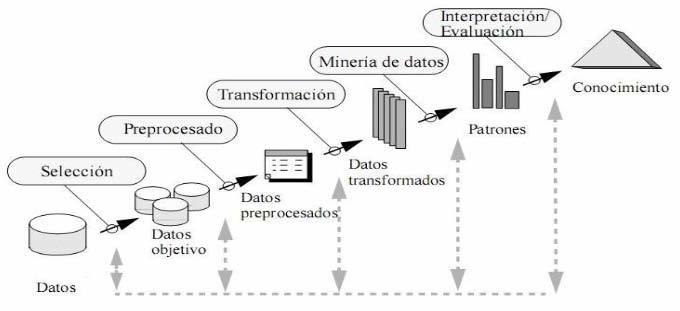
\includegraphics[width=4.06111in,height=2.68611in]{img/KDD.png}
  \caption{Flujo gráfico KDD}
  \label{fig:flujo_kdd}
\end{figure}

Al seguir la metodología KDD, nos aseguraremos de seguir un enfoque sistemático y riguroso para el análisis de los datos recopilados, lo que nos permitirá obtener conocimientos significativos y relevantes relacionados con la resolución de la guía de programación, el éxito académico y la deserción estudiantil en el curso de Introducción a la Programación en la Universidad Andrés Bello.


\subsection{Descripción de la base de datos}

En esta investigación, se utiliza un conjunto de datos que registra a los estudiantes que tomaron el 
curso de Introducción a la Programación en la Universidad Andrés Bello durante el año 2021. 
Estos datos incluyen información sobre el rendimiento de los estudiantes en la resolución de la guía de apoyo para la primera evaluación.

La base de datos cuenta con un total de 839 registros que registran información detallada de los 
estudiantes, y se compone de 75 columnas que contienen diversas variables relacionadas con el curso 
y el desempeño de los estudiantes.

\begin{table}[htbp]
  \centering
  \caption{Descripción de variables}
  \begin{tabular}{|l|p{0.6\linewidth}|}
    \hline
    \textbf{Variable}              & \textbf{Descripción}                                                                                                                                                               \\
    \hline
    sol1                           & Indica la calificación obtenida en la primera evaluación, con un valor binario donde 1 indica una respuesta correcta a la pregunta, mientras que el valor predeterminado es 0. \\
    \hline
    exitosos                       & Indica la cantidad de preguntas respondidas correctamente en la guía.                                                                                                          \\
    \hline
    fallidos                       & Indica la cantidad de preguntas respondidas incorrectamente en la guía.                                                                                                        \\
    \hline
    hito1                          & Son las espectativas a cumplir del aprendizaje del curso.                                                                                                                          \\
    \hline
    hito2                          & Son las espectativas a cumplir del aprendizaje del curso.                                                                                                                          \\
    \hline
    programa                       & Indica al programa de estudio.                                                                                                                                                 \\
    \hline
    Columnas de la e0 hasta la e52 & Son las preguntas respondidas de la guia este es binario.                                                                                                                          \\
    \hline
  \end{tabular}
  \label{tab:variables}
\end{table}


Estas columnas son relevantes para nuestro análisis, ya que nos permitirán examinar la relación 
entre la resolución de la guía de programación, el éxito académico en la primera evaluación y 
el programa de estudio al que pertenecen los estudiantes (véase Tabla \ref{tab:variables}).



\subsection{Recopilación de datos}

Para llevar a cabo este estudio, se cuenta con el conjunto de datos denominado "dataset a 2021", que contiene la información necesaria sobre los
resultados de la guía de programación y el rendimiento en la primera evaluación del curso de Introducción a la Programación en el año 2021.


\subsection{Análisis de datos}

Una vez recopilados los datos, se realizará un análisis descriptivo para examinar la distribución de los resultados en la guía de programación y
la primera evaluación. Además, se llevará a cabo un análisis de correlación entre las variables mencionadas anteriormente para identificar posibles
relaciones y patrones significativos.


\hypertarget{analisis_resultado}{%
    \section{Análisis Resultado}\label{Análisis Resultado}}

En nuestro analisis de resultado, se revisará la relación entre la resolución de la guía de programación y el éxito académico en el ramo de introducción a la programación. Se analizará específicamente la columna exitosos del conjunto de datos dataset a 2021, con el objetivo de responder a la pregunta de investigación planteada en este estudio: ¿La resolución de una guía de programación está relacionada con el éxito académico en el ramo de introducción a la programación en la Universidad Andrés Bello? De esta manera, se podrá determinar si resolver la guía es actualmente significativo para predecir el rendimiento en la solemne 1 del año 2021,

\subsection{Descripción del DataFrame}

La tabla \ref{tab:descripcion_dataframe} presenta una descripción del DataFrame, que incluye información sobre las columnas, el número de valores no nulos y los tipos de datos correspondientes. Analizando esta descripción, podemos obtener una visión general de la estructura y las características del DataFrame.

\begin{table}[htbp]
    \centering
    \caption{Descripción del DataFrame}
    \begin{tabular}{lll}
        \hline
        \textbf{Columna} & \textbf{Non-Null Count} & \textbf{Dtype} \\
        \hline
        hito1            & 839 non-null            & float64        \\
        hito2            & 839 non-null            & float64        \\
        exitosos         & 839 non-null            & int64          \\
        fallidos         & 839 non-null            & int64          \\
        sol1             & 839 non-null            & float64        \\
        aprobado         & 839 non-null            & int64          \\
        e0 - e52         & 839 non-null            & int64          \\
        \hline
    \end{tabular}%
    \label{tab:descripcion_dataframe}%
\end{table}%

En la tabla \ref{tab:descripcion_dataframe}, cada una de estas columnas tiene un total de 839 valores no nulos y se identifica el tipo de dato correspondiente. Estos detalles son fundamentales para comprender la composición y las propiedades del DataFrame analizado.

\subsection{Estadísticas de la variable sol1}

En el análisis de datos, es importante comprender las características estadísticas de las variables numéricas. En este contexto, hemos examinado la variable sol1 y recopilado estadísticas como el recuento, la media, la desviación estándar, los cuartiles y el sesgo. Estos valores nos proporcionan información sobre la distribución y la tendencia central de la variable.

En la tabla \ref{tab:estadistica_variable_sol1}, la variable "sol1" presenta una media de aproximadamente 3.6 y una desviación estándar de alrededor de 1.83. La distribución de los datos muestra una ligera asimetría positiva con un sesgo de aproximadamente 0.03. Estos resultados nos ayudan a comprender la variabilidad y la forma de la distribución de la variable sol1.

\begin{table}[htbp]
    \centering
    \caption{Estadísticas de la variable sol1}
    \begin{tabular}{ll}
        \hline
        \textbf{Medida}    & \textbf{Valor}       \\
        \hline
        Count              & 839.000000           \\
        Mean               & 3.642789             \\
        Standard Deviation & 1.832625             \\
        Minimum            & 1.000000             \\
        25\% Percentile    & 2.200000             \\
        50\% Percentile    & 3.700000             \\
        75\% Percentile    & 5.100000             \\
        Maximum            & 7.000000             \\
        Skewness           & 0.033079652062595215 \\
        \hline
    \end{tabular}%
    \label{tab:estadistica_variable_sol1}%
\end{table}%



\subsection{Coeficiente de asimetría}

El coeficiente de asimetría es una medida estadística que nos proporciona información sobre la asimetría de una distribución de datos. En el contexto de los datos analizados, hemos obtenido un coeficiente de asimetría de aproximadamente 3.31\%. Este valor indica una ligera asimetría positiva en la distribución.

\begin{table}[htbp]
    \centering
    \caption{Coeficiente de asimetría}
    \begin{tabular}{ll}
        \hline
        \textbf{Coeficiente de asimetría}      & \textbf{Valor}       \\
        \hline
        Coeficiente de asimetría               & 0.033079652062595215 \\
        Coeficiente de asimetría en porcentaje & 3.31\%               \\
        \hline
    \end{tabular}%
    \label{tab:skewness}%
\end{table}%

En la tabla \ref{tab:skewness}, se puede apreciar la aproximacion de 0.033079652062595215 lo cual nos indica que la distribución de los datos tiene una ligera asimetría hacia la derecha. Esto implica que hay una cola derecha más larga en comparación con la cola izquierda de la distribución. En términos porcentuales, esta asimetría representa aproximadamente el 3.31\% del rango total de la distribución.

\subsection{Coeficiente de Variación}

El coeficiente de variación es una medida de la dispersión relativa de una variable en relación a su media. Nos permite evaluar la variabilidad de los datos en comparación con su valor promedio. Se calcula dividiendo la desviación estándar por la media y se expresa como un porcentaje.

\begin{table}[htbp]
    \centering
    \caption{Coeficiente de Variación}
    \begin{tabular}{ll}
        \hline
        \textbf{Medida}                        & \textbf{Valor}     \\
        \hline
        Coeficiente de Variación               & 0.5027829289053924 \\
        \hline
        Coeficiente de Variación en Porcentaje & 50.28\%            \\
        \hline
    \end{tabular}%
    \label{tab:coef_variacion}%
\end{table}%

En la tabla \ref{tab:coef_variacion}, se muestra el coeficiente de variación calculado para los datos analizados. El coeficiente de variación es de aproximadamente 0.5027, lo que indica una alta dispersión relativa en relación con la media. Esto se confirma por el coeficiente de variación en porcentaje, que es del 50.28\%. Estos resultados destacan la variabilidad de los datos en el conjunto de datos analizado.

\subsection{Obteniendo Amplitud}

La amplitud es una medida de la variabilidad o dispersión de los datos. Nos permite evaluar la diferencia entre el valor máximo y mínimo de una variable, proporcionando información sobre la extensión de los datos en el conjunto.

\begin{table}[htbp]
    \centering
    \caption{Amplitud}
    \begin{tabular}{ll}
        \hline
        \textbf{Medida} & \textbf{Valor}     \\
        \hline
        Amplitud        & 0.5600809456082252 \\
        \hline
    \end{tabular}%
    \label{tab:amplitud}%
\end{table}%

En la tabla \ref{tab:amplitud}, se muestra la amplitud calculada para los datos analizados. La amplitud es de aproximadamente 0.56\%, lo que indica la diferencia entre el valor máximo y mínimo de la variable. Esta medida nos proporciona una idea de la extensión de los datos en el conjunto analizado.

\subsection{Tabla de Frecuencias}

Utilizando los datos obtenidos de la tabla \ref{tab:skewness} y la tabla \ref{tab:amplitud}, se ha construido una tabla de frecuencias que muestra la distribución de los datos en intervalos. Los intervalos se definen con base en
la amplitud y el valor máximo de los datos analizados.

\begin{table}[htbp]
    \centering
    \caption{Tabla de Frecuencias}
    \begin{tabular}{lllll}
        \hline
        \textbf{Intervalo} & \textbf{f\_i} & \textbf{F\_i} & \textbf{h\_i} & \textbf{H\_i} \\
        \hline
        (0.0, 0.56]        & 0             & 0             & 0.000000      & 0.000000      \\
        (0.56, 1.12]       & 152           & 152           & 0.181168      & 0.181168      \\
        (1.12, 1.68]       & 21            & 173           & 0.025030      & 0.206198      \\
        (1.68, 2.24]       & 66            & 239           & 0.078665      & 0.284863      \\
        (2.24, 2.8]        & 79            & 318           & 0.094160      & 0.379023      \\
        (2.8, 3.36]        & 34            & 352           & 0.040524      & 0.419547      \\
        (3.36, 3.92]       & 103           & 455           & 0.122765      & 0.542312      \\
        (3.92, 4.48]       & 76            & 531           & 0.090584      & 0.632896      \\
        (4.48, 5.04]       & 87            & 618           & 0.103695      & 0.736591      \\
        (5.04, 5.6]        & 81            & 699           & 0.096544      & 0.833135      \\
        (5.6, 6.16]        & 53            & 752           & 0.063170      & 0.896305      \\
        (6.16, 6.72]       & 57            & 809           & 0.067938      & 0.964243      \\
        \hline
    \end{tabular}%
    \label{tab:tabla_frecuencias}%
\end{table}%

En la tabla \ref{tab:tabla_frecuencias}, se presenta la tabla de frecuencias que muestra la cantidad de datos en cada intervalo, el total acumulado de datos hasta ese intervalo, la frecuencia relativa del intervalo y la frecuencia
relativa acumulada. Esta tabla nos permite visualizar la distribución de los datos y su acumulación en cada intervalo.

El intervalo más relevante en esta tabla es el intervalo (3.36, 3.92], ya que contiene la mayor frecuencia (103) y la mayor acumulación (455). Esto indica que la mayoría de los datos se encuentran en este rango de valores.

A continuación, se muestra una nueva tabla con información adicional:

\begin{table}[htbp]
    \centering
    \caption{Información adicional}
    \begin{tabular}{lllll}
        \hline
        \textbf{Mediana} & \textbf{Intervalo de la mediana} & \textbf{Máximo} & \textbf{Intervalo del máximo} \\
        \hline
        3.7              & $f_i$ 103.000000                 & 7.0             & $f_i$ 57.000000               \\
                         & $F_i$ 455.000000                 &                 & $F_i$ 809.000000              \\
                         & $h_i$ 0.122765                   &                 & $h_i$ 0.067938                \\
                         & $H_i$ 0.542312                   &                 & $H_i$ 0.964243                \\
        \hline
    \end{tabular}%
    \label{tab:informacion_adicional}%
\end{table}%

En la tabla \ref{tab:informacion_adicional}, se muestra la mediana de los datos, así como el intervalo en el que se encuentra dicha mediana. Además, se indica el valor máximo y el intervalo en el que se encuentra dicho valor máximo.

\subsection{Histograma con curva de densidad}

El histograma con curva de densidad es una herramienta visual importante en el análisis de datos para comprender la distribución de los valores de la variable sol1.

\begin{figure}[htbp]
    \centering
    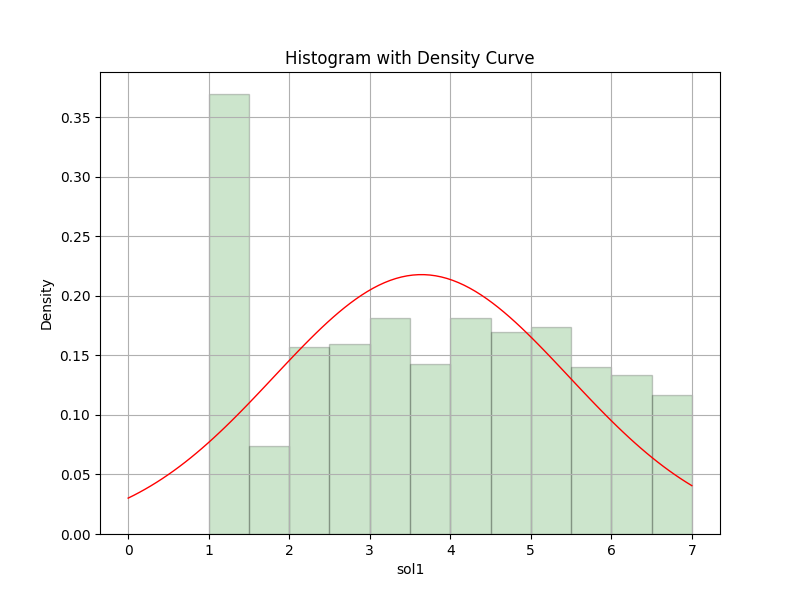
\includegraphics[width=4.06111in,height=2.68611in]{img/histogramaConCurvaDeDensidad.png}
    \caption{Histograma con Curva de Densidad}
    \label{fig:hist_density}%
\end{figure}%


La figura \ref{fig:hist_density} muestra este tipo de gráfico correspondiente a los datos analizados.

En el eje Y se presentan los valores de densidad que van desde 0.00 hasta aproximadamente 0.35, representando la densidad de la variable sol1. Por otro lado, en el eje X se muestran los valores del 0 al 7, que representan las diferentes notas obtenidas en la columna sol1 (solemne 1).

La mayor concentración de datos se encuentra alrededor del valor 0.35 en el eje Y, lo cual indica que la mayoría de las observaciones tienen una nota baja en sol1.

La curva de densidad, representada en color rojo, alcanza su punto más alto entre las notas 3 y 4 en el eje X. Esta curva suavizada muestra la forma general de la distribución de los valores de sol1. A medida que las notas aumentan, la densidad disminuye gradualmente.

En resumen, el análisis del histograma con curva de densidad revela que la mayoría de las observaciones tienen una nota baja en sol1, concentrándose principalmente alrededor del valor 0.35 en el eje Y. Además, la curva de densidad muestra un pico más alto entre las notas 3 y 4 en el eje X.

\subsection{Identificar valores atípicos}

En el análisis de datos, la detección de valores atípicos es crucial para identificar observaciones que difieren significativamente de la tendencia general. Estos valores pueden tener un impacto significativo y requerir atención especial.

A continuación se muestra una tabla con los valores atípicos identificados mediante el método del Z-score. Se calculó el Z-score para cada observación utilizando un umbral de 3 desviaciones estándar. Los valores que superan este umbral se consideran atípicos y se presentan en la tabla:

\begin{table}[htbp]
    \centering
    \caption{Valores Atípicos}
    \begin{tabular}{ccccccc}
        \hline
        \textbf{hito1} & \textbf{hito2} & \textbf{exitosos} & \textbf{fallidos} \textbf{programa} & \textbf{sol1} & \textbf{aprobado}     \\
        21.0           & 6.0            & 17                & 14                                  & UNAB11500     & 1.0               & 0 \\
        2.0            & 2.0            & 4                 & 27                                  & UNAB12210     & 1.0               & 0 \\
        4.0            & 4.0            & 6                 & 41                                  & UNAB12510     & 1.5               & 0 \\
        0.0            & 0.0            & 0                 & 47                                  & UNAB12100     & 1.6               & 0 \\
        10.0           & 6.0            & 9                 & 38                                  & UNAB11500     & 1.6               & 0 \\
        12.0           & 0.0            & 9                 & 38                                  & UNAB12210     & 2.4               & 0 \\
        42.0           & 12.0           & 26                & 37                                  & UNAB21500     & 2.5               & 0 \\
        32.0           & 32.0           & 26                & 5                                   & UNAB11500     & 3.4               & 0 \\
        9.0            & 0.0            & 7                 & 40                                  & UNAB11500     & 4.3               & 1 \\
        38.0           & 6.0            & 28                & 35                                  & UNAB12210     & 4.4               & 1 \\
        32.0           & 32.0           & 26                & 5                                   & UNAB12210     & 4.6               & 1 \\
        18.0           & 2.0            & 11                & 20                                  & UNAB12210     & 4.6               & 1 \\
        32.0           & 14.0           & 21                & 10                                  & UNAB12210     & 5.9               & 1 \\
        13.0           & 25.0           & 16                & 15                                  & UNAB22115     & 7.0               & 1 \\
        7.0            & 0.0            & 5                 & 42                                  & UNAB12100     & 7.0               & 1 \\
        \hline
    \end{tabular}%
    \label{tab:valores_atipicos}%
\end{table}%

Observando los valores atípicos en la tabla \ref{tab:valores_atipicos}, podemos notar que algunas observaciones difieren significativamente en al menos una de las variables. "Exitosos" representa las respuestas correctas de la guía, "Fallidos" indica la cantidad de errores para lograr los "Exitosos", y "Envíos" es la suma de "Exitosos" y "Fallidos". "Sol1" se refiere a la nota obtenida en la solemne 1. Estos valores atípicos pueden ser de interés para un análisis más detallado, ya que podrían indicar situaciones excepcionales o errores en la recolección de datos.

\hypertarget{Conclusiones}{%
    \section{Conclusiones}\label{Conclusiones}}

A lo largo de esta investigación, hemos emprendido un viaje analítico en el que las herramientas modernas, como SHAP y DoWhy, se han convertido en aliados esenciales para desentrañar las complejidades del rendimiento estudiantil. La naturaleza multidimensional del rendimiento académico exige un enfoque que no solo identifique correlaciones, sino que también desentrañe las relaciones causales que subyacen en estos patrones.

Un aspecto crucial de nuestra investigación fue la comparación exhaustiva de diferentes algoritmos, tanto de clasificación como de regresión. Esta comparación nos permitió adentrarnos en el proceso de selección del mejor modelo para llevar a cabo nuestras predicciones con SHAP. Gracias a este análisis detallado, pudimos identificar y seleccionar el algoritmo óptimo que no solo proporcionó precisión en las predicciones, sino que también ofreció una mayor interpretabilidad al analizar la importancia de las características.

Nuestros hallazgos revelan la importancia de variables como \texttt{hito1}, \texttt{exitosos}, \texttt{fallidos} y \texttt{e29} en el contexto académico. No obstante, lo que hace que esta investigación sea particularmente reveladora no es solo la identificación de estas variables, sino la comprensión de cómo interactúan y afectan el rendimiento de los estudiantes. La capacidad de SHAP para descomponer la importancia predictiva de cada variable ha sido crucial, proporcionando insights que van más allá de la mera correlación.

Por su parte, DoWhy nos ha permitido explorar el mundo de la causalidad, aportando una nueva dimensión a nuestro análisis. Más allá de saber qué variables son importantes, ahora comprendemos mejor \textit{por qué} son importantes y cómo pueden influir activamente en el rendimiento académico.

Con base en nuestros descubrimientos, se sugiere que futuras investigaciones en este ámbito consideren proporcionar relaciones más detalladas entre variables como \texttt{hito1} y las preguntas específicas de la guía que pertenecen a este hito. Además, incorporar información adicional como la asistencia a clases, el sexo, la edad, entre otras, podría enriquecer significativamente el análisis. Específicamente, herramientas como SHAP podrían utilizarse para visualizar el impacto de estas variables adicionales y entender su relación con la probabilidad de aprobación.

Finalmente, es esencial reconocer que, aunque nuestros hallazgos son robustos y prometedores, aún existen factores externos no controlados que pueden influir en la respuesta de un alumno a una guía o en su rendimiento general. La incorporación de variables adicionales y la continuación de este tipo de análisis permitirán reducir la incertidumbre y mejorar la precisión de nuestras predicciones.

En conclusión, esta investigación no solo ha arrojado luz sobre las dinámicas del rendimiento estudiantil, sino que también ha establecido un camino para futuras investigaciones. Mediante el uso combinado de análisis predictivo y causal, podemos aspirar a desarrollar estrategias educativas más informadas y efectivas, siempre con el objetivo de mejorar la experiencia y el éxito académico de los estudiantes.

%%%%%%%%%%%%%%%%%%%%%%%%%%%%%%%%%%%%%%%%%%%%%%%%%%%%%%%%%%%%%%%%%%%%%%%%%%%%%%%

%%%%%%%%%%%%%%%%%%%%%%%%%%%%%%% bibliografia %%%%%%%%%%%%%%%%%%%%%%%%%%%%%%%%
    \printbibliography
%%%%%%%%%%%%%%%%%%%%%%%%%%%%%%%%%%%%%%%%%%%%%%%%%%%%%%%%%%%%%%%%%%%%%%%%%%%%%%%

    
\end{document}